\chapter{Proposed System Titles}
\ifpdf
    \graphicspath{{Chapter2/Chapter2Figs/PNG/}{Chapter2/Chapter2Figs/PDF/}{Chapter2/Chapter2Figs/}}
\else
    \graphicspath{{Chapter2/Chapter2Figs/EPS/}{Chapter2/Chapter2Figs/}}
\fi

\section{Proposed System Title}
%\markboth{}{\MakeUppercase{\thechapter. Proposed System Title }}
\markboth{}{Node Failures and its Impact on Data Aggregation Delay}{}

\subsection{Subsection1}
You can write contents for your subsection here...

\subsection{Subsection2}

You can write contents for your subsection here...

\begin{table}[ht]
\caption{The Symbols Used in the Paper} % title of Table
\centering % used for centering table
\begin{tabular}{l p{9cm}} % centered columns (4 columns)
\hline\hline %inserts double horizontal lines
Symbol & Description \\ [0.5ex] % inserts table
%heading
\hline % inserts single horizontal line
$N$ & Amount of SNs in tree WSN \\ % inserting body of the table
$m$ & Amount of INs in tre WSN \\
$T_{comp}$ & Time taken for comparing two sensed values \\
$T_{net}$ & Transmission time from one wireless node to another in the WSN \\
\hline %inserts single line
\end{tabular}
\label{table:table1} % is used to refer this table in the text
\end{table}

The total energy consumed by the GN is proportional to the amount of computations and amount of transmissions. The total delay or energy consumed or time taken by the GN to complete the aggregate computation in a balanced two level tree WSN is,

\begin{equation}
T_{max} = {\frac{N}{m}-1}
\end{equation}

\begin{figure}[t] %inserts the figure at the top of the page t denotes the top of the page %[!htbp]
  \begin{center}
    \leavevmode  
      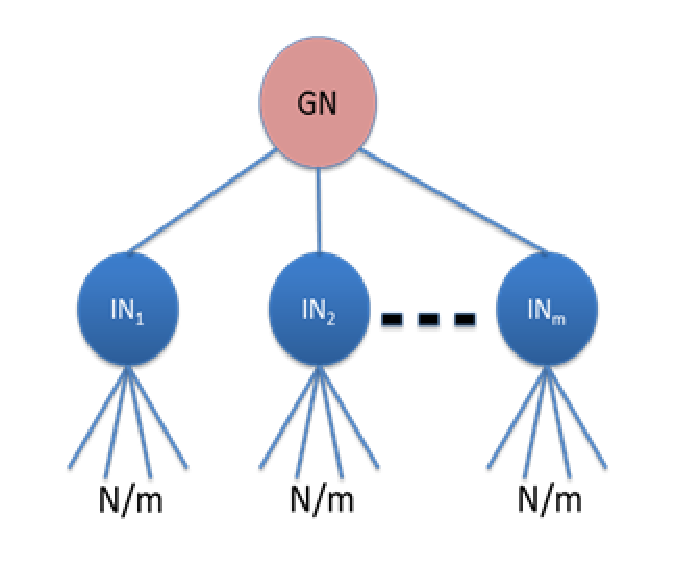
\includegraphics[height=2in]{5.eps}
     \caption{Balanced Two Level Tree WSN}     
    \label{bal}
  \end{center}
\end{figure}

% ------------------------------------------------------------------------

%%% Local Variables: 
%%% mode: latex
%%% TeX-master: "../thesis"
%%% End: 
